% Source: Weinberg GR, physical PDF p. 470 (printed p. 447).
% Coverage: Figure 14.11, radio galaxy 3C295 and its spectrum.
% Status: source photograph and spectrograph extracted at source resolution;
%         source-reviewed and compile-clean.
% Uncertainties: none.

\begingroup
\renewcommand{\thefigure}{14.11}
\begin{figure}[htbp]
  \centering
  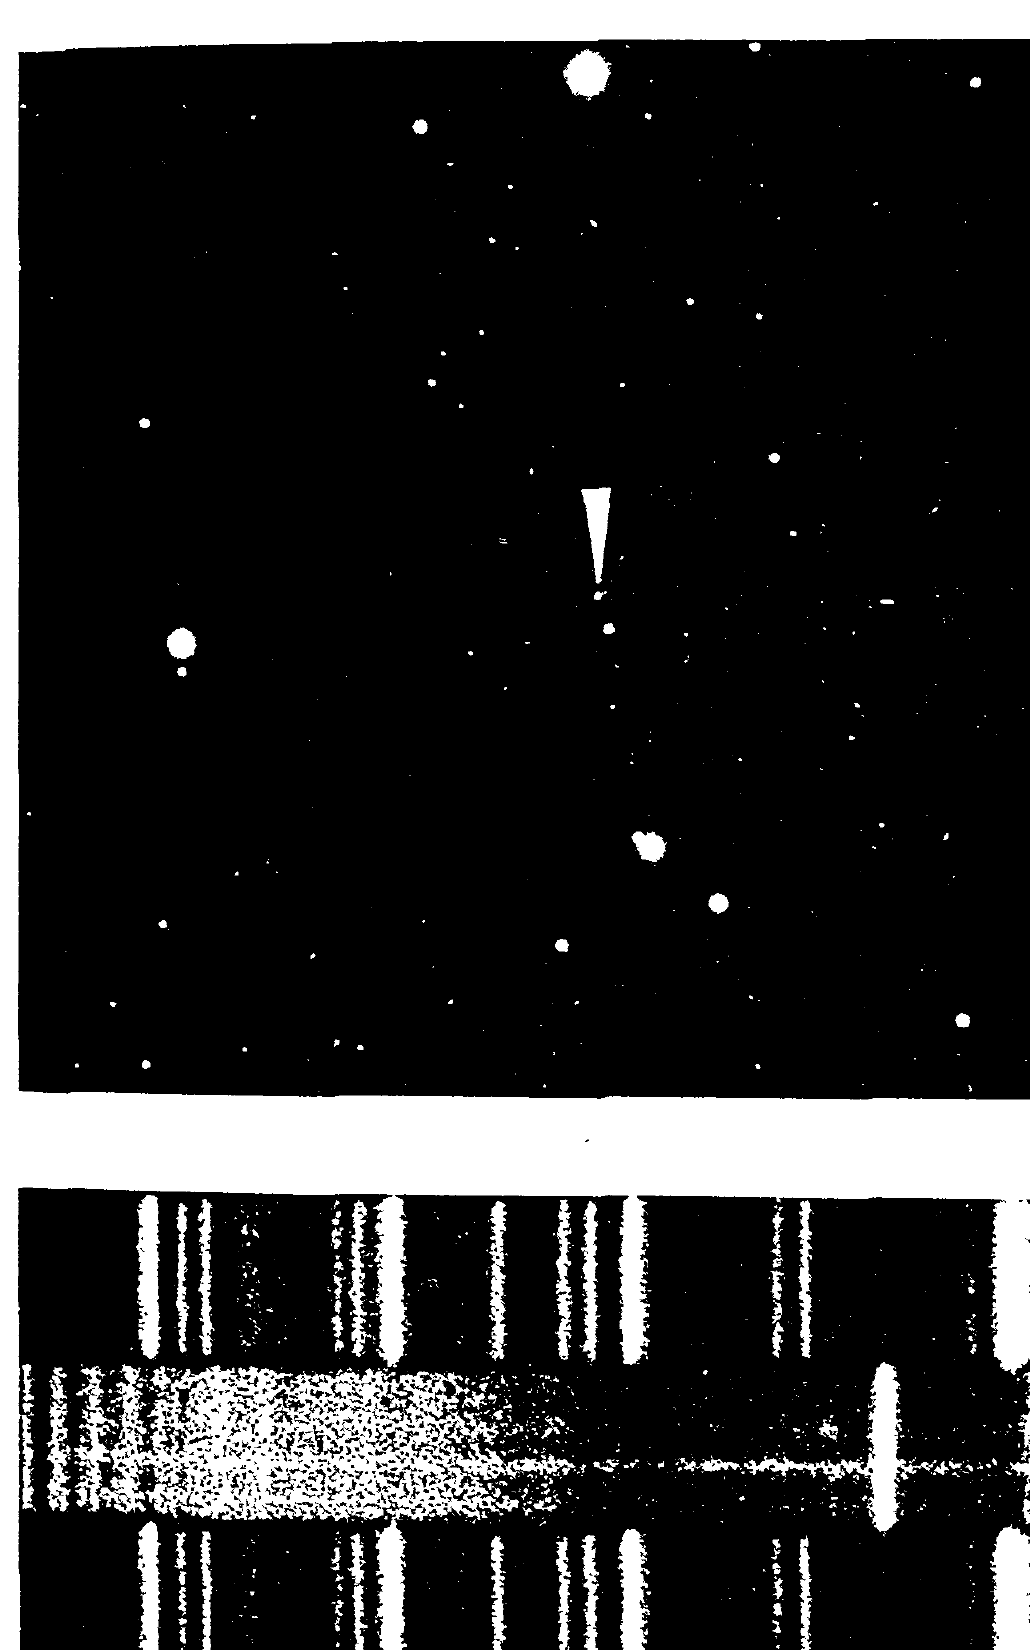
\includegraphics[height=0.68\textheight]{figures/chapter14/fig14-11.png}
  \caption{The radio galaxy 3C295 in Boötes. The spectrum of this galaxy,
  shown below, reveals a red shift \(z=0.46\), the largest yet observed for
  any galaxy. This photograph and spectrograph were taken with the 200-in.\
  telescope at Mt.\ Palomar. (Courtesy Mt.\ Wilson and Mt.\ Palomar
  observatories.)}
  \label{fig:14.11}
\end{figure}
\endgroup
